\documentclass {article}

% example taken from 
% http://www.guitex.org/home/images/doc/GuideGuIT/introingtikz.pdf
\usepackage[utf8]{inputenc}
\usepackage[british]{babel}
\usepackage[sc]{mathpazo}
\usepackage[T1]{fontenc}


% Or whatever. Note that the encoding and the font should match. If T1
% does not look nice, try deleting the line with the fontenc.
% \usepackage{lmodern} %optional

\usepackage{parskip,amsmath,array,booktabs,amssymb,color,alltt,bm,colortbl,bigints,wasysym,a4wide} 

\usepackage{mathtools}
\addtolength{\topmargin}{-15mm}

\newcommand{\iid}{\mbox{\,$\perp\!\!\!\perp$\,}}
\DeclareMathOperator{\logit}{logit}
\DeclareMathOperator{\E}{\mathbb{E}}
\DeclareMathOperator{\V}{\mathbb{V}}
\DeclareMathOperator{\C}{\mathbb{C}}
\DeclareMathOperator{\argmax}{\arg\max}
\DeclareMathOperator{\tr}{tr}
\DeclareMathOperator{\R}{\bfseries\textsf{R}}

\newcommand{\mc}[3]{\multicolumn{#1}{#2}{#3}}  
\newcommand{\bx}{\ensuremath{\bm{x}}}
\newcommand{\bbx}{\ensuremath{\bar{\bx}}}
\newcommand{\tbx}{\ensuremath{\tilde{\bx}}}
\newcommand{\bu}{\ensuremath{\bm{u}}}
\newcommand{\bv}{\ensuremath{\bm{v}}}
\newcommand{\bmf}{\ensuremath{\bm{f}}}
\newcommand{\bep}{\ensuremath{\bm{\varepsilon}}}
\newcommand{\by}{\ensuremath{\bm{y}}}
\newcommand{\bym}{\ensuremath{{\bm{y}_\text{mis}}}}
\newcommand{\byo}{\ensuremath{{\bm{y}_\text{obs}}}}
\newcommand{\bz}{\ensuremath{\bm{z}}}
\newcommand{\bmu}{\ensuremath{\bm{\mu}}}
\newcommand{\Sm}{\ensuremath{\Sigma}}
\newcommand{\Lm}{\ensuremath{\Lambda}}
\newcommand{\lm}[1]{\ensuremath{\lambda_{#1}}}
\newcommand{\Lmt}{\ensuremath{\Lm\Lm^\top}}
\newcommand{\diff}[1]{\ensuremath{{\frac{\partial}{\partial#1}}}}
\newcommand{\difff}[2]{\ensuremath{{\frac{\partial^2}{\partial#1\partial#2}}}}
\newcommand{\N}{\ensuremath{\mathcal{N}}}
\newcommand{\be}[1]{\ensuremath{{\bm{e}_{(#1)}}}}
\newcommand{\bt}{\ensuremath{{\bm{\theta}}}}
\newcommand{\bti}[1]{\ensuremath{{\bm{\theta}^{(#1)}}}}
\newcommand{\setfont}[1]{\fontsize{#1pt}{#1pt}\selectfont}
\newcommand{\code}[1]{{\texttt{#1}}}

\usepackage {tikz}
\usetikzlibrary {positioning}
%\usepackage {xcolor}
\definecolor {processblue}{cmyk}{0.96,0,0,0}
\begin {document}
\section*{Eksamensopgave 3 spørgsmål 5}
Vi tager udgangspunkt i DAG'en fra tidligere
\begin {center}
\begin {tikzpicture}[-latex ,auto ,node distance =3 cm and 3cm ,on grid ,
semithick ,
state/.style ={ circle ,top color =white  ,
	draw , text=black , minimum width =1 cm}]
\node[state] (S){$S$};
\node[state] (B) [below right=of S] {$B$};
\node[state] (L) [below =of S] {$L$};
\node[state] (X) [below left=of L] {$X$};
\node[state] (D) [below=of B] {$D$};
\path (S) edge [] node[] {} (X);
\path (S) edge [] node[] {} (L);
\path (S) edge [] node[] {} (B);
\path (L) edge [] node[] {} (X);
\path (B) edge [] node[] {} (D);
\path (L) edge [] node[] {} (D);
%\path (A) edge [bend right = -15] node[below =0.15 cm] {$1/2$} (C);
%\path (A) edge [bend left =25] node[above] {$1/4$} (B);
%\path (B) edge [bend left =15] node[below =0.15 cm] {$1/2$} (A);
%\path (C) edge [bend left =15] node[below =0.15 cm] {$1/2$} (B);
%\path (B) edge [bend right = -25] node[below =0.15 cm] {$1/2$} (C);
\end{tikzpicture}
\end{center}
Først moraliserer vi den, altså fjerner retningen på kanterne og gifter alle forældre

\begin {center}
\begin {tikzpicture}[auto ,node distance =3 cm and 3cm ,on grid ,
semithick ,
state/.style ={ circle ,top color =white  ,
	draw , text=black , minimum width =1 cm}]
\node[state] (S){$S$};
\node[state] (B) [below right=of S] {$B$};
\node[state] (L) [below =of S] {$L$};
\node[state] (X) [below left=of L] {$X$};
\node[state] (D) [below=of B] {$D$};
\path (S) edge [] node[] {} (X);
\path (S) edge [] node[] {} (L);
\path (S) edge [] node[] {} (B);
\path (L) edge [] node[] {} (X);
\path (B) edge [] node[] {} (D);
\path (L) edge [] node[] {} (D);
\path (L) edge [] node[] {} (B);
\end{tikzpicture}
\end{center}
Grafen skal nu trianguleres, men det er den allerede, så vi går direkte videre til at identificering af kliker.
\begin{figure}[h]
	\begin{center}
		\scriptsize
		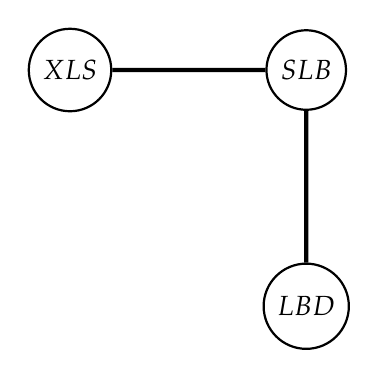
\begin{tikzpicture}[scale=1.5, shape=circle, minimum size = 1cm, thick] 
		\node (XLS) at  ( 0, 2) [draw] {$XLS$};
		\node (SLB) at ( 2, 2) [draw] {$SLB$};
		\node (LBD) at  ( 2, 0) [draw] {$LBD$};
		\draw[line width=1.5pt] (XLS) -- (SLB);
		\draw[line width=1.5pt] (SLB) -- (LBD);     
		\end{tikzpicture}  
	\end{center}
\end{figure}
Vi laver nu et kliketræ eller som det hedder på engelsk junction tree
\begin{figure}[h]
	\begin{center}
		\scriptsize
		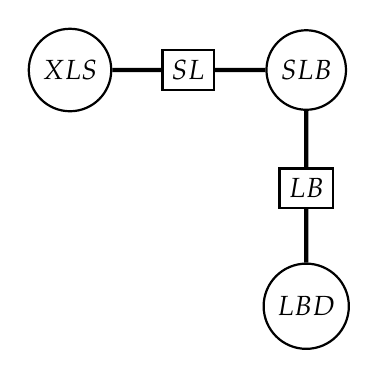
\begin{tikzpicture}[scale=1.5, shape=circle,  minimum size = .5cm, thick] 
		\node (XLS) at  ( 0, 2) [draw] {$XLS$};
		\node (SLB) at ( 2, 2) [draw] {$SLB$};
		\node (LBD) at  ( 2, 0) [draw] {$LBD$};
		\node (SL)   at ( 1, 2) [rectangle,draw] {$SL$};
		\node (LB)  at ( 2, 1) [rectangle,draw] {$LB$};    
		\draw[line width=1.5pt] (XLS) -- (SL);
		\draw[line width=1.5pt] (SL) -- (SLB);
		\draw[line width=1.5pt] (SLB) -- (LB);
		\draw[line width=1.5pt] (LB) -- (LBD);
		\end{tikzpicture}  
	\end{center}
\end{figure}
Ud fra det vi tidligere er kommet frem til at simultanfordelingen er givet ved
\begin{align*}
	P(V)&=P(S,B,L,X,D)\\
	&=P(S)P(L|S)P(X|L,S)P(B|S)P(D|L,B)
\end{align*}
Den kan vi nu nemmere regne ud med \[ P(V)=q_1(X,L,S)q_2(S,L,B)q_3(L,B,D) \]
Som vi deler op således
\begin{align*}
	q_1(X,L,S)=P(S)P(X|L,S)\\
	q_2(S,L,B)=P(L|S)P(B|S)\\
	q_3(L,B,D)=P(D|L,B)
\end{align*}
\end{document}
